\section{Apps}
\begin{frame}
\note<1>{Um mit git zu arbeiten, gibt es verschieden Tools}
\begin{itemize}
	\item<2-> SmartGit, SourceTree, …
	\item<3-> GitHub Desktop
	\item<4-> Integriert in Visual Studio Code
\end{itemize}
\end{frame}

\subsection{SmartGit, SourcTree und Co}
\begin{frame}
\note<1>{Ein paar Worte zu…}
\begin{itemize}
\item<2-> Umfassende GUIs
\item<3-> Erweiterte Funktionalitäten über GUI:
\begin{itemize}
\item<4-> cherry picking
\item<5-> Konfliktlösungen
\item<6-> …
\end{itemize}
\end{itemize}
\end{frame}

\subsection{SmartGit}
\begin{frame}
\begin{center}
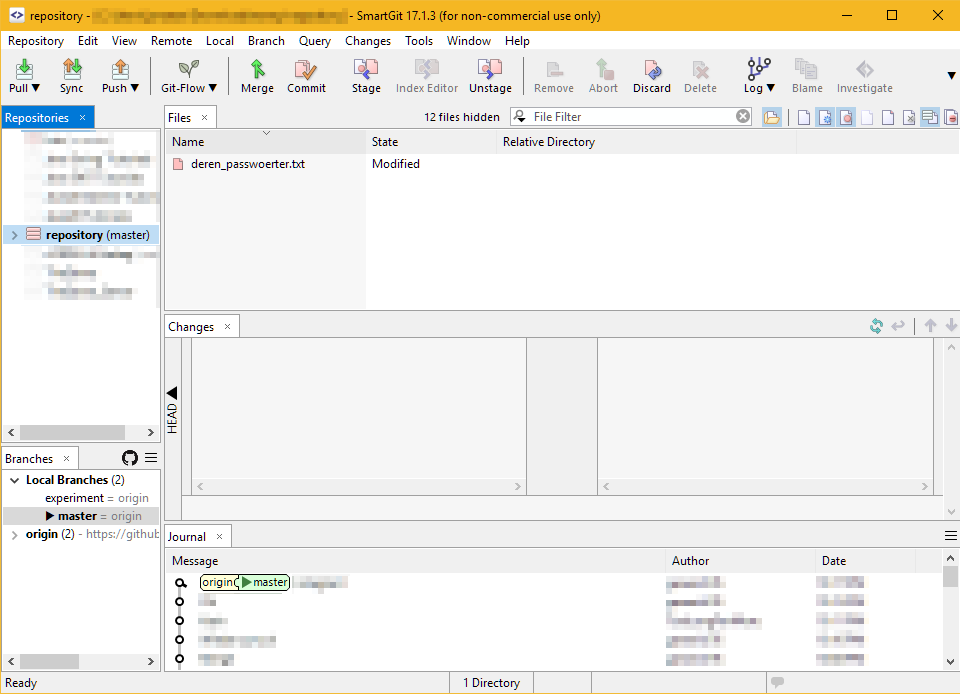
\includegraphics[scale=.4]{bilder/smartgit.png}
\end{center}
\end{frame}

\subsection{SourceTree}
\begin{frame}
\begin{center}
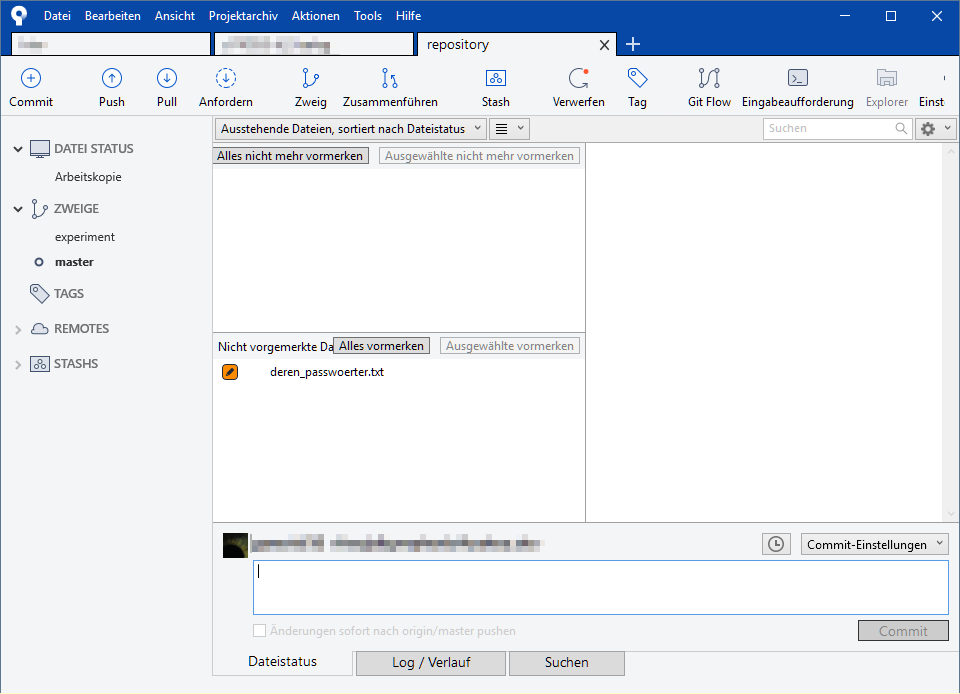
\includegraphics[scale=.4]{bilder/sourcetree.png}
\end{center}
\end{frame}

\subsection{GitHub Desktop}
\begin{frame}
\note<1>{Wenn man sowieso mit github arbeitet…}
\begin{itemize}
\item<2-> Sehr eingeschränkte Funktionalität
\item<3-> Für Alltag ausreichend
\end{itemize}
\end{frame}

\begin{frame}
\begin{center}
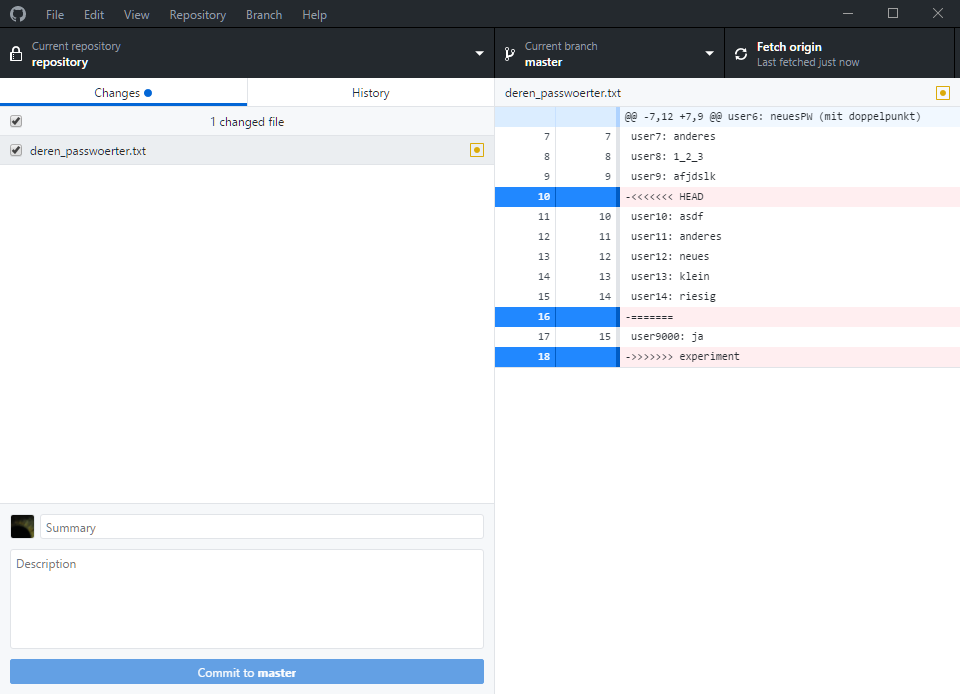
\includegraphics[scale=.4]{bilder/githubdesktop.png}
\end{center}
\end{frame}

\subsection{Visual Studio Code}
\begin{frame}
Features:
\begin{itemize}
	\item <2->Einbindung in Entwicklungsumgebung
	\begin{itemize}
		\item <3->Direkter Import (clone) von Git Repositories
		\item <4->Grundlegende Befehle sind verfügbar
%		\item <5->Automatische file checkouts
		\note{beim Rückgängig machen}
	\end{itemize}
	\item <5->Anzeige aktuell geänderter Passagen im Editor
\end{itemize}
\end{frame}